\begin{figure}[H]
	\begin{center}
		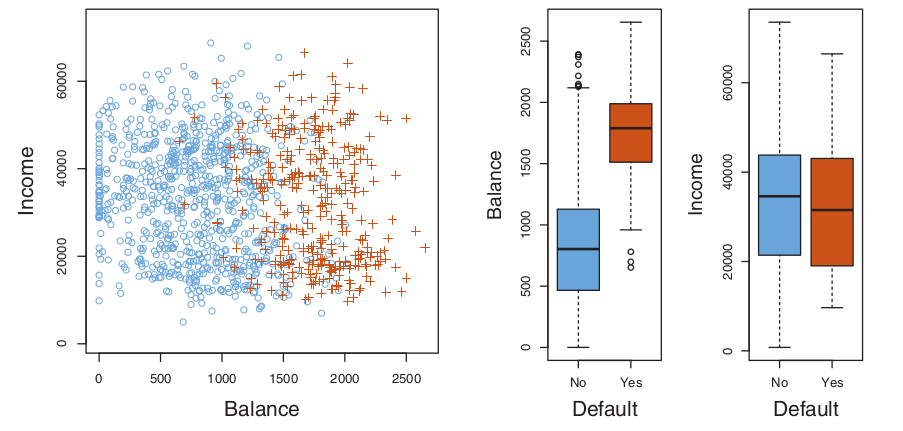
\includegraphics[width=\textwidth]{./chap/1chap/3sec/1images/1DefaultDataSetPlot.png}
	\end{center}
	\caption{The \emph{default} data set.\\Left:indivduals who
defaulted in orange in a given month and those who did not in blue.\\}
Right: The first boxplot shows the balance distribution split by the
binary default variable, the second plot the income distribution.
	\label{fig:fig3.1}
\end{figure}
It appears that individuals who defaulted tended to have a higher 
credit card balances.\\In this chapter we learn how to build a model to
predict default for  any values of balance and income.
